\subsection{\underline{DSR}}%\underline{\textbf{DSR}}\\
    Comme \textit{AODV}, \textit{DSR} est un protocole réactif à vecteur de distance.\\
    % ack lors de la reception d'un paquet
    Deux mécanismes principaux caractérisent \textit{DSR}\\
    \begin{enumerate}
        \item \textbf{Route Discovery}\\
            Similaire à la découverte de chemins dans AODV. La différence est que le \textit{RREQ} va contenir l'id de tous les sauts de chemin.\\
            Quand la cible d'un \textit{RREQ} le reçoit, elle va répondre avec un \textit{RREP} contenant le chemin du \textit{RREQ} inversé.\\
            Les paquets de données contiennent le chemin complet par lequel ils doivent transiter.\\
            On a donc des paquets d'une taille variant avec celle du chemin emprunté.
        \item \textbf{Route Maintenance}\\
            Chaque noeud est responsable des liens entre lui et ses successeurs et possède une cache de routes.
            Pour cela, quand un noeud reçoit un paquet, il va transmettre à la source de ce paquet
            un \textit{ack}. Si le \textit{ack} n'est pas reçu au bout d'un temps fixé, l'émetteur du paquet va émettre
            un paquet \textit{route\_error} à ses prédécesseurs pour leur signaler que le lien n'existe plus.\\
            Si des routes sont interrompues, les noeuds peuvent soit utiliser d'autres routes de leur cache, soit initier une \textit{route discovery}
    \end{enumerate}
    \begin{figure}[H]
        \centering
        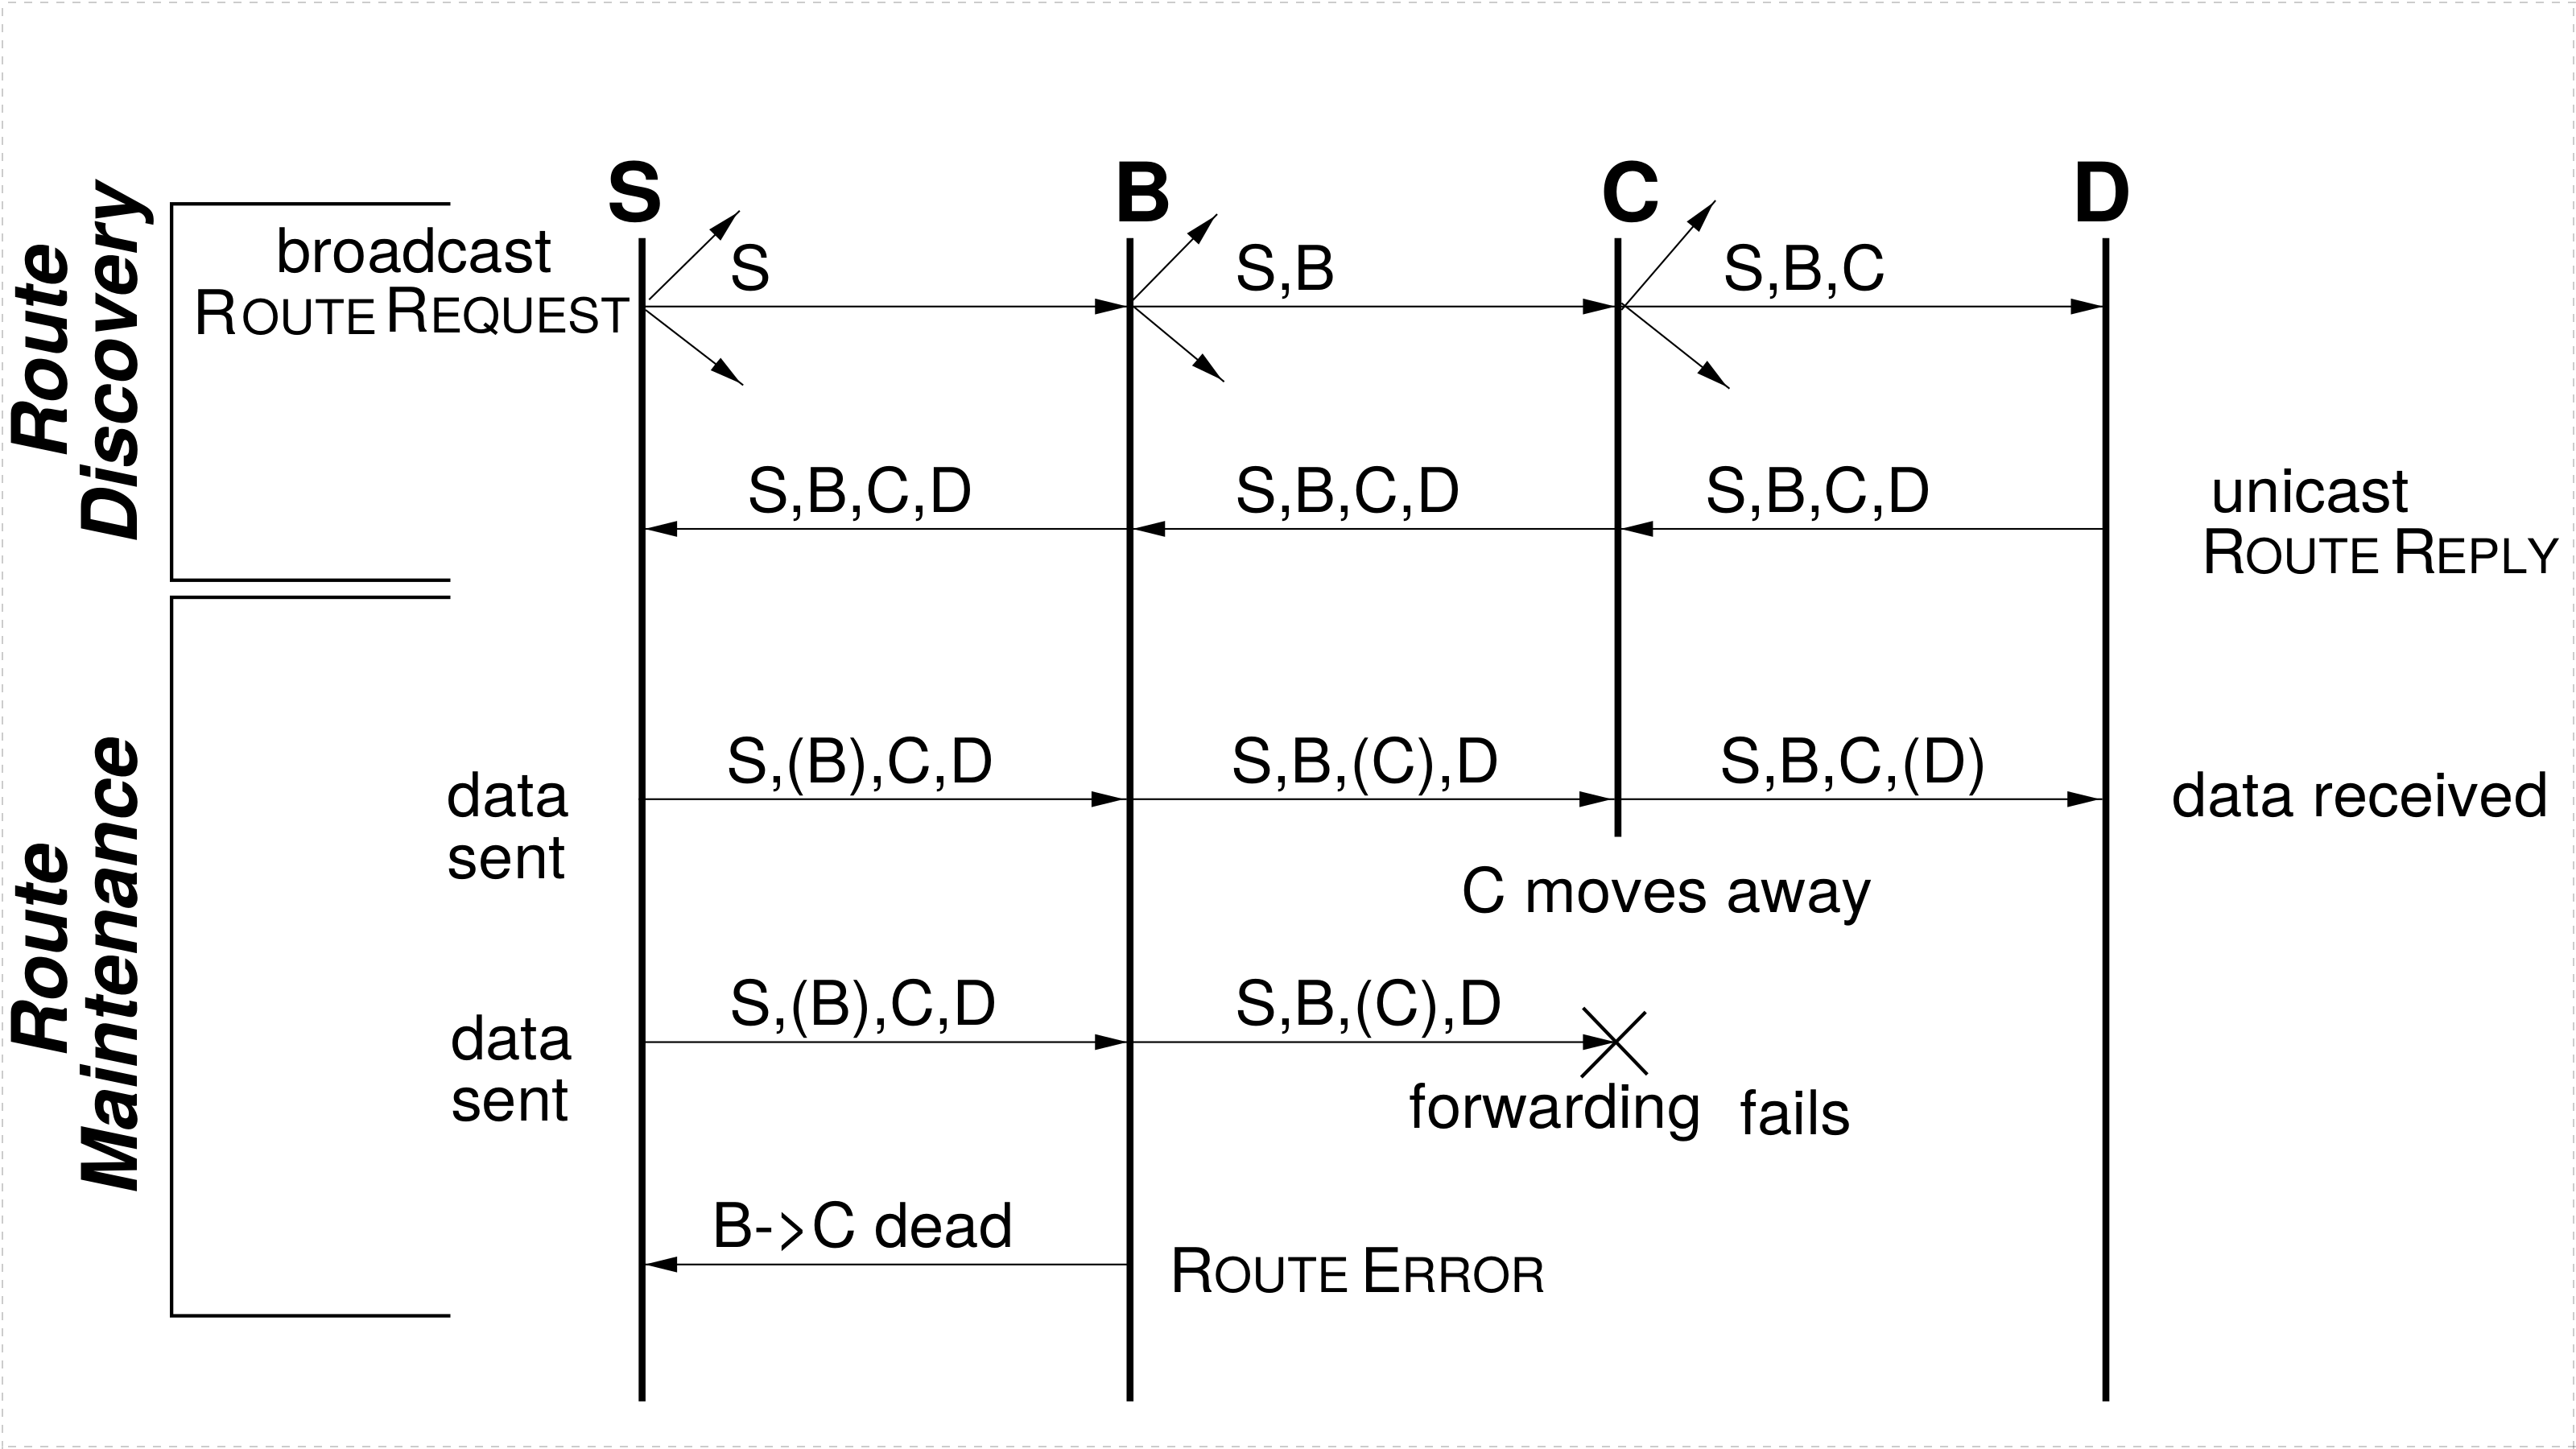
\includegraphics[scale=0.12]{images/ack_dsr.png}
        \caption{Illustration de DSR \cite{dsr_for_adHoc_network}}
        \label{dsr_image}
    \end{figure}